% ----------------------------------------------------------------------------
\chapter{Analysis and Comparison of Chat Systems}
\label{chatsystems}
In my analysis of chat systems, I will start with
the Internet Relay Chat (IRC). It seems a natural starting point for me,
as I am still an extensive user of this chat system for historical reasons.
What worries me is its low security standard, which I will briefly describe.
I will then turn to SILC, which has been developed to address IRC weakness
regarding security. Secure message delivery has ben its main
innovation. XMPP is of special interest, because it has been designed as an
open and adaptive chat system featuring a high level of decentralisation.
The last chat system in this comparison is Skype, the only commercial
system analysed. Due to its questionable development history and present, it is
a controversially viewed chat system, albeit with a huge user base.
I will end this chapter by giving an overview of omitted chat systems
and a comparison of the security features.
%%    1. Detailed analysis and comparison of open and legacy chat systems
%%        to summarise current chat system features and their
%%        security characteristics.
% ----------------------------------------------------------------------------
\section{Internet Relay Chat (IRC)}
\subsection{History}
IRC has been developed since 1989 and was first formally documented in May 1993 in 
RFC 1459\cite{rfc1459}. It is still being widely used.\cite{ircusage}
The current protocol is specified in the RFCs 2810-2813\cite{rfc2810,rfc2811,rfc2812,rfc2813}.
%%\begin{quote}
%%All client-to-server IRC protocols in use today are descended from the protocol implemented in the irc2.4.0 version of the IRC2 server, and documented in RFC 1459. Since RFC 1459 was published, the new features in the irc2.10 implementation led to the publication of several revised protocol documents (RFC 2810, RFC 2811, RFC 2812 and RFC 2813); however, these protocol changes have not been widely adopted among other implementations.\ref{irc-wp}
%%\end{quote}
% ----------------------------------------------------------------------------
\subsection{Architecture}
IRC is organised centrally, as stated in \cite{rfc2810}:
\begin{quote}
The IRC protocol provides no mean for two clients to directly
communicate.  All communication between clients is relayed by the
server(s).
\end{quote}
There is, however, an unofficial client extension named 
\textit{Direct Client-to-Client (DCC)}\cite{dcc,ctcp}
available in most IRC clients that enables direct connections.
Figure \ref{ircoverview} shows the schematic overview of an IRC network.
\begin{figure}
    \caption{Schematic Overview of IRC}
    \label{ircoverview}
    \centering
    
    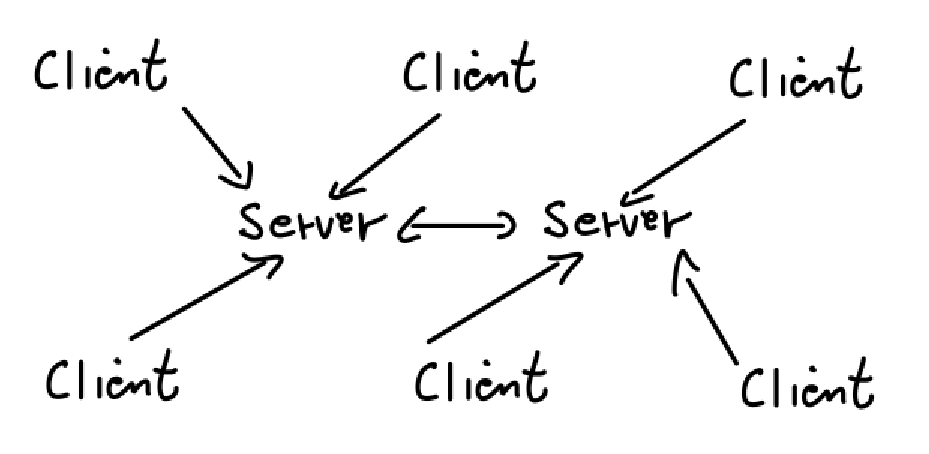
\includegraphics{irc.eps}
\end{figure}
IRC supports 
\textit{direct chat} (one peer to another peer) as well 
as \textit{group chat} (many peers to many peers). The group chat is
realised by creating \textit{IRC channels}, sometimes also called 
\textit{chat rooms}.
% ----------------------------------------------------------------------------
\subsection{Security}
In general, all communications are based on a plaintext protocol.
The TLS protocol \cite{rfc2246} is being used for encryption
in some networks, but its use is not standardised. 
Connections from clients to servers
as well as servers to servers may be encrypted.
Some networks support special channel modes to ensure all connected peers
use an encrypted connection. There is no such mode for
direct chat. For normal IRC channels, there is no guarantee that all
peers are connected using an encrypted connection.

Due to this architecture, every server operator can listen to all
messages, even if encryption is being used. As the network usually consists
of many clients, but only a small number of servers, an attacker needs
to concentrate on a small number of victim hosts only.

Usually IRC networks do not provide any kind of anonymisation features:
every user can request detailed information about other users, including
their IP address.  The freenode network\cite{freenode} however,
supports so called \textit{cloaks}, which transform the IP address information
into a generic string like \textit{gpm/telmich}, in which gpm describe the
project and telmich the name. There are various other cloaking expressions
available.
% ----------------------------------------------------------------------------
\section{Secure Internet Live Conferencing (SILC)}
% ----------------------------------------------------------------------------
\subsection{History}
The \textit{Secure Internet Live Conferencing (SILC)} protocol
has been developed by Pekka Riikonen since 1996. The first public release
was made in 2000. The latest releases of SILC software (server and client)
date back to 2009. SILC can be considered a more secure successor of IRC,
as can be seen in the following quote:
\begin{quote}
\ldots{}
Many of the SILC features are found in traditional chat protocols such 
as IRC but many of the SILC features can also be found in 
Instant Message (IM) style protocols.

SILC combines features from both of these chat protocol styles, 
and can be implemented as either IRC-like system 
or IM-like system. \ldots{}\cite{silcwp}
\end{quote}
As far as the official website reports,
there is no version controlled source code repository available,
only tarballs from 2009 are download-able. This may indicate that the
development of the SILC software has stalled.
% The SILC Project's goal is to fully standardize the SILC protocol in the IETF. 
%Bug form does not return any bugs.
Besides the official SILC Network, which is run by 7 SILC servers,
there are about 12 other SILC networks being run.\cite{wiki:silc}
% ----------------------------------------------------------------------------
\subsection{Architecture}
Figure \ref{silcoverview} shows 
that SILC network architecture looks similar to the IRC network architecture: 
\begin{figure}
    \centering
    \caption[Schematic Overview of SILC]{Schematic Overview of SILC\\Image source: \protect\url{http://www.silcnet.org/img/silc_network.png}}
    \label{silcoverview}
    \includegraphics[scale=0.8]{silc_network.png}
\end{figure}
Both rely on a central design orientated on a network of servers.
In case of SILC, there are two different variants of message passing:
\begin{itemize}
\item Private Message Delivery With Session Keys
\item Private Message Delivery With Private Message Key
\end{itemize}
In any case, all messages are travelling through supporting servers and are never
transmitted directly from one to another client.
% ----------------------------------------------------------------------------
\subsubsection{Private Message Delivery With Session Keys}
When the SILC client uses session keys, every message is send encrypted
with the session key of the next peer, decrypted at the peer and re-encrypted
for the next peer in the chain, as can be seen in figure \ref{silcsessionkey}.
\begin{figure}
    \centering
    \caption[Silc: Private Message Delivery With Session Keys]{Private Message Delivery With Session Keys\\Image source: \protect\url{http://www.silcnet.org/img/silc_priv1.png}}
    \label{silcsessionkey}
    \includegraphics[scale=0.8]{silc_priv1.png}
\end{figure}
In this scenario, every peer in the communication chain
can read the content of the message.
% ----------------------------------------------------------------------------
\subsubsection{Private Message Delivery With Private Message Key}
When using a a private message key, the servers in the communication chain
only forward the message and the receiving peer is the only one who can
decrypt the message. Figure \ref{silcprivkey} illustrates this behaviour.
\begin{figure}
    \centering
    \caption[Silc: Private Message Delivery With Private Message Key]{Private Message Delivery With Private Message Key\\Image source: \protect\url{http://www.silcnet.org/img/silc_priv2.png}}
    \label{silcprivkey}
    \includegraphics[scale=0.8]{silc_priv2.png}
\end{figure}
% ----------------------------------------------------------------------------
\subsection{Security}
As all messages in the SILC network are encrypted, an external attacker
cannot read the message content. In case private message delivery with session keys
is utilised, a compromised SILC server may be used to intercept and read all
messages. This is not possible, if messages are sent using
private message delivery with private message key.
Due to the small number of servers (7 in the official network),
an attacker could run a \textit{Denial-of-Service (DoS)} attack to prevent
users from chatting.

The SILC network does not provide any kind of anonymity services and allows
to query detailed information about a peer including the IP address.
% ----------------------------------------------------------------------------
\section{Extensible Messaging and Presence Protocol (XMPP)}
% ----------------------------------------------------------------------------
\subsection{History}
The \textit{Extensible Messaging and Presence Protocol (XMPP)}
was originally developed by Jeremie Miller in 1998 and released
to the public as \textit{Jabber} in 1999. In 2004 Jabber
was transferred to the IETF, renamed to XMPP
and is now defined in several
RFCs\cite{rfc3920,rfc3921,rfc3922,rfc3923,rfc4622,rfc4854,rfc4979,rfc6120,rfc6121}.
Since then, the \textit{XMPP Standards Foundation (XSF)} is responsible
for standardising XMPP related protocols, the so called 
\textit{XMPP Extension Protocols (XEP)}.
By 2003 XMPP has been used by an estimated 10 million people\cite{xmppuser}.
AOL added experimental support for XMPP in the 
\textit{AOL instant Messenger (AIM)} in 2008.
In 2010 the social-networking site Facebook added support for
third-party applications via XMPP.
As of 2012, there are over 30 different client and about 20
server implementations available.
% ----------------------------------------------------------------------------
\subsection{Architecture}
The XMPP network is built upon the ideas of e-mail: Users are identified
by e-mail like usernames like \textit{nico@example.org}. The clients and
servers find the correct server to talk to by making a
DNS SRV\cite{rfc2782} look-up. 
Clients are asking for the \textit{xmpp-client} service and
servers are asking for the \textit{xmpp-server} service.
Thus a client may ask for a SRV record
\url{_xmpp-client._tcp.example.net.} or a server for
\url{_xmpp-server._tcp.im.example.com.}
If there is no SRV record, the client or server can fall back
to request for the A or AAAA record, similar to how 
SMTP\cite{rfc2821} behaves. Figure \ref{jabberarch} shows
how the client \textit{nico@example.org} sends a message
to \textit{nico@example.net}.
\begin{figure}
    \centering
    \caption{XMPP Network Architecture}
    \label{jabberarch}
    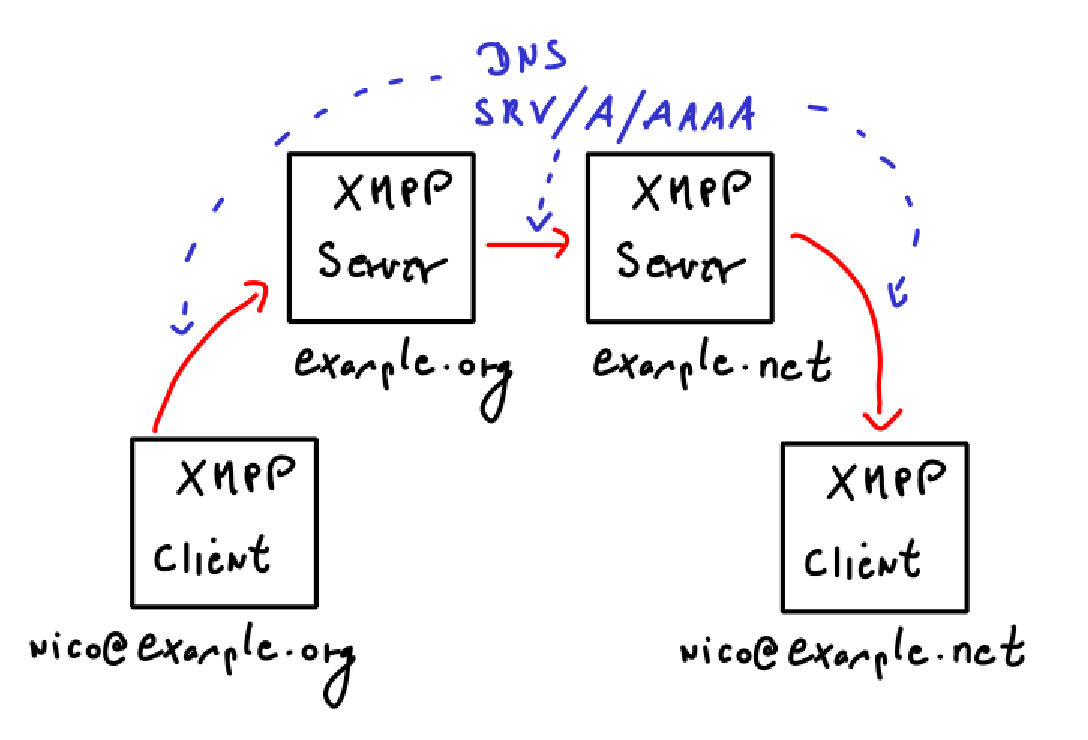
\includegraphics[scale=0.8]{jabberarch.eps}
\end{figure}
XMPP formats messages based on the 
\textit{Extensible Markup Language (XML)} and
supports authentication using the
Simple Authentication and Security Layer (SASL)\cite{rfc4422}.
Clients never talk directly to each other in a XMPP network, but
always use one or more servers in between. Compared to IRC and SILC,
XMPP is the only protocol that supports connecting other protocols
like AIM or IRC.
% ----------------------------------------------------------------------------
\subsection{Security}
Within XMPP, TLS is being used for encryption and SASL for authentication.
XMPP does not have a mechanism to support anonymity.
To create a DoS attack, an attacker can choose to take either the sending
or the receiving server down. Due to its openness, an attacker can find out
which server needs to be attacked by doing DNS queries. Though when attacking
the sending server, the sending client can just switch to another server,
as figure \ref{jabbersendingserverattack} shows.
\begin{figure}
    \centering
    \caption{XMPP Sending Server Attack}
    \label{jabbersendingserverattack}
    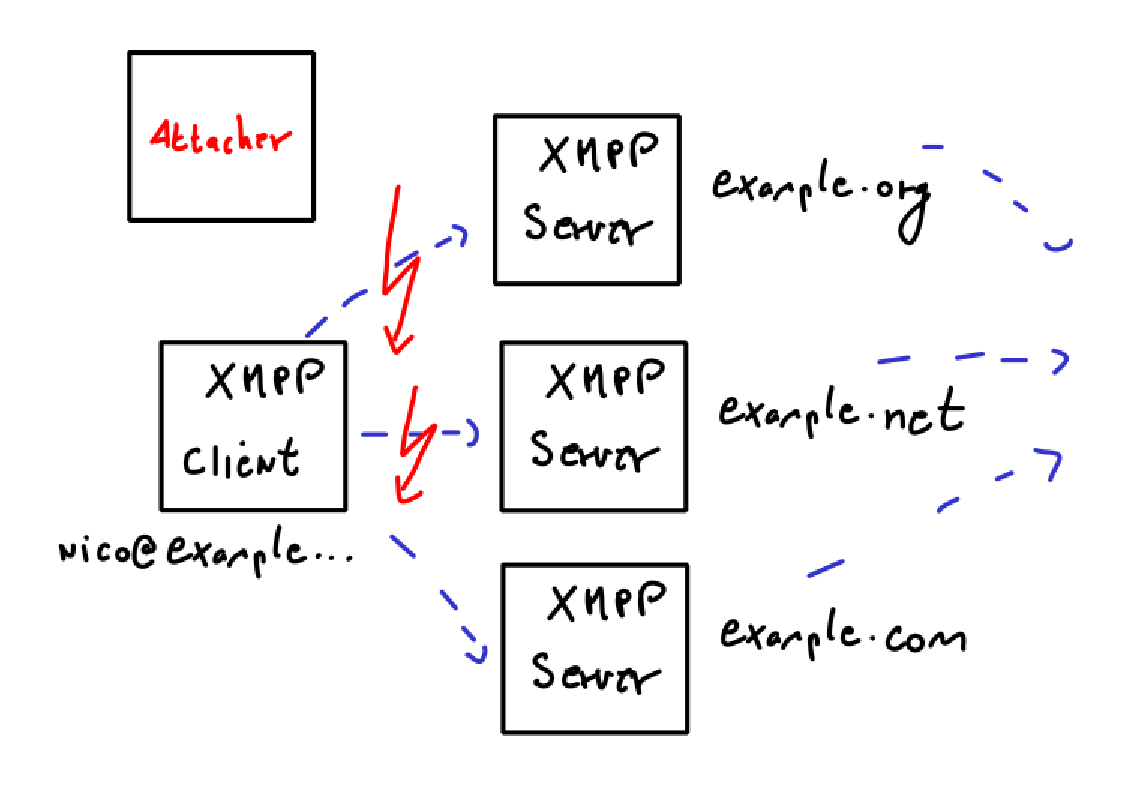
\includegraphics[scale=0.7]{jabbersendingserverattack.eps}
\end{figure}
If the attacker aims to bring down the receiving server, the message
will not arrive while the server is down, as shown in figure 
\ref{jabberreceivingserverattack}.
\begin{figure}
    \centering
    \caption{XMPP Receiving Server Attack}
    \label{jabberreceivingserverattack}
    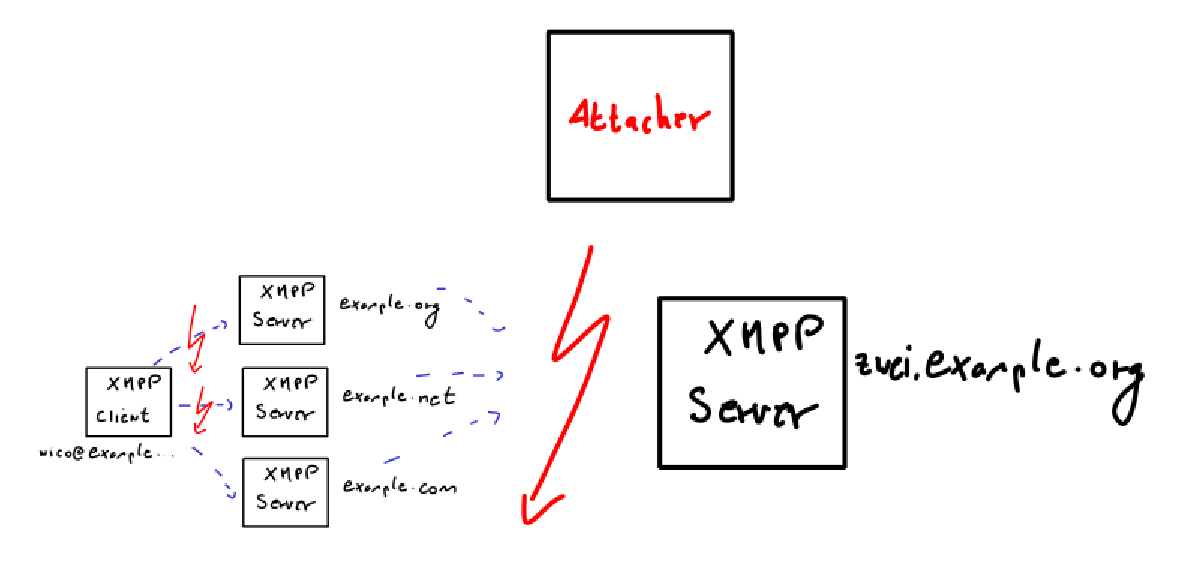
\includegraphics[scale=0.7]{jabberreceivingserverattack.eps}
\end{figure}
% ----------------------------------------------------------------------------
\section{Skype}
% ----------------------------------------------------------------------------
\subsection{History}
The following excerpt\cite{wiki:skype} gives a rough overview of Skype's history:
\begin{quote}
Skype was founded in 2003 by Janus Friis from Denmark and Niklas Zennström from Sweden.
The Skype software was developed by Estonians Ahti Heinla, Priit Kasesalu, and Jaan Tallinn, 
who together with Janus and Niklas were also behind the peer-to-peer file sharing software 
Kazaa. In August 2003, the first public beta version was released.
\end{quote}
In April 2006, the number of registered users reached 100 million.
In July 2010 several online newspapers announced that a hacker from the USA
has successfully managed to reverse engineer the
protocol. The suspected results can be found on \cite{skype:source}.
In May 2011 Microsoft acquired Skype. There are various efforts made to 
keep up the reverse engineering of the program and the 
protocol, some driven by Russian scientists. During the research
of this thesis multiple websites referencing protocol details have been
made inaccessable, some of them were replaced by a website that claimed
that the content is prohibited by the Digital Millennium Copyright Act (DMCA).
Skype as of today is being used on many computers and mobile phones.

There is also a variant of Skype available called TOM, which has been produced
for the Chinese market after Skype's initial banning from the China.
%% http://www1.cs.columbia.edu/~library/TR-repository/reports/reports-2004/cucs-039-04.pdf
%% 
%% 
%% http://www.heise.de/newsticker/meldung/Skype-unter-die-Lupe-genommen-111559.html
%% 
%% 
%% http://www.secdev.org/conf/skype_BHEU06.handout.pdf
%% 
%% 
%% 
%% In January 2011, after the release of video calling on the Skype client for iPhone, Skype reached a record 27 million simultaneous online users.[45] This record was broken with 29 million simultaneous online users on 21 February 2011,[46] and again on 28 March 2011 with 30 million online users.[47] On 25 February 2012, Skype announced that it has over 32 million users for the first time ever.[48]. As of 05 March 2012, it has broken to 35 million simultaneous online users.[49]
%% 
%% 
%% % ----------------------------------------------------------------------------
\subsection{Architecture}
Skype's network is a mixture of a centralised and peer-to-peer network.
As figure \ref{skypearch} shows, it consists of three entities:
\begin{itemize}
\item Supernodes
\item Ordinary Nodes
\item Login Servers
\end{itemize}
The function of these three nodes is explained in \cite{skype-analysis}:
\begin{quote}
An ordinary host is
a Skype application that can be used to place voice calls and send
text messages. A super node is an ordinary host’s end-point on the
Skype network. Any node with a public IP address having
sufficient CPU, memory, and network bandwidth is a candidate to
become a super node. An ordinary host must connect to a super
node and must register itself with the Skype login server for a
successful login. Although not a Skype node itself, the Skype
login server is an important entity in the Skype network.
\end{quote}
In case a client is behind a firewall that does
\textit{network address translation (NAT)}, 
Skype uses a variant of STUN\cite{rfc5389}.
\begin{figure}
    \centering
    \caption[Skype Network Architecture]{Skype Network Architecture a (Image source: \cite{skype-analysis})}
    \label{skypearch}
    \includegraphics[scale=0.8]{skype-network.png}
\end{figure}
In contrast to the previous three protocols, Skype use is more focused on voice chat.
The connection is encrypted using AES-256, the keys are encrypted using
1536 up to 2048 Bit RSA.
Furthermore, variants of RC4 are being used, which may be attackable.
The website describing this attack is not reachable anymore, but 
is still quoted
on Wikipedia.\footnote{\url{http://www.enrupt.com/index.php/2010/07/07/skype-biggest-secret-revealed}}
% ----------------------------------------------------------------------------
\subsection{Security}
Although Skype makes use of secure encryption methods (AES, RSA), it has
various other security threads: The software itself is programmed to detect
debugging scenarios and contains encrypted code. This may led to the
assumption that the Skype developers are trying to hide information from the
user. Although Skype is reported to support encryption between the two
communicating peers\cite{skype:encrypted}, at least the Chinese variant TOM
supports surveillance operations:\cite{skype-tom}
\begin{quote}
The full text chat messages of TOM-Skype users, along with Skype users who have
communicated with TOM-Skype users, are regularly scanned for sensitive keywords, and
if present, the resulting data are uploaded and stored on servers in China.

These text messages, along with millions of records containing personal information, are
stored on insecure publicly-accessible web servers together with the encryption key required to
decrypt the data.

The captured messages contain specific keywords relating to sensitive political topics such
as Taiwan independence, the Falun Gong, and political opposition to the Communist Party
of China.

Our analysis suggests that the surveillance is not solely keyword-driven. Many of the
captured messages contain words that are too common for extensive logging, suggesting
that there may be criteria, such as specific usernames, that determine whether messages are
captured by the system.
\end{quote}
As the non-TOM Skype binary itself is encrypted, it is possible that it contains similar
functions.
Another uncertainty is caused by statements of government agencies, which
claim to be able to intercept all Skype traffic.
Skype is treated
similarly as traditional phone companies, which indicates truth of the given
statements.
Furthermore recent reports
indicate that Microsoft changes the supernode structure so that instead of having
supernodes at the user, the supernodes reside centrally at Microsoft's
datacenters to allow easy wiretapping.\cite{skype:supernodechange}
%% Skype konnte schon zuvor durch Ermittlungsbehörden abgehört werden.[8]
%% Austrian public broadcasting service ORF, citing minutes from the meeting, reported that "the Austrian police are able to listen in on Skype connections". Skype declined to comment on the reports.
% ----------------------------------------------------------------------------
\section{Other}
There are further chat protocols, which have not been included into this
analysis, either because of known weaknesses, irrelevance or small user base.
ICQ, which has been published in 1996, is not being widely used anymore
and its protocol, OSCAR\cite{oscar}, is based on plain text messages.
ICQ used to be popular, but has been sold to the Russian Mail.ru group.
Furthermore the old \textit{Microsoft Messenger protocol (MSN)} has not
been taken into account.
% ----------------------------------------------------------------------------
\section{Security features and Comparison}
The different chat systems and their architectures have shown a variety
of strengths and weaknesses, which are summarised in the table below.
\begin{longtable}{|c|c|c|c|c|}
\caption{Chat system comparison with security features}\\
\hline
\textbf{Name} & \textbf{IRC} & \textbf{SILC} & \textbf{XMPP} & \textbf{Skype}\\
\hline
\textbf{Central server architecture} & yes & yes & no & yes/no\footnote{Supernodes take a special role and are
being centralised by Microsoft's work.}\\
\hline
\textbf{Encrypted messages} & optional & yes & yes & yes\\
\hline
\textbf{Anonymity Support} & yes/no\footnote{IP address cloaking}  & yes/no\footnote{IP address cloaking} & no & no\\
\hline
\textbf{Proprietary Protocol} & no  & no & no & yes\\
\hline
\textbf{Software owned by one (commercial) company} & no  & no & no & yes\\
\hline
\textbf{Network being run by one (commercial) company} & no  & no & no & yes\\
\hline
\textbf{Source Code accessible} & yes  & yes & yes & no\\
\hline
\textbf{Encrypted binary software} & no  & no & no & yes\\
\hline
\end{longtable}
%% To summarise:
%% \begin{itemize}
%% \item Anonymity support is only 
